\documentclass[12pt,a4paper]{article}
 
\usepackage{float}
%für feststellen der figures und tables [H] dranschreiben
\usepackage{units}
%wird so benutzt: 
%\unit[value/Zahl]{dimension/Einheit} oder 
%\unitfrac[value/Zahl]{dimension/Einheit num/Zähler}{dimension/Einheit denum/Nenner} oder
%\nicefrac[fontcommand/Schriftart]{dimension/Einheit num/Zähler}{dimension/Einheit denum/Nenner}

\usepackage{caption}
\usepackage{subcaption}

\usepackage{listings}		% Wird für Quelltext verwendet

\usepackage[left=2cm,right=2cm,top=2cm,bottom=2cm]{geometry}
\usepackage[utf8]{inputenc}
\usepackage[T1]{fontenc}
\usepackage{lmodern}
\usepackage[ngerman]{babel}
\usepackage{amsmath}
\usepackage{graphicx}
 
%niemals zwei überschriften direkt übereinander schreiben, also immer mindestens in einem satz was sinnvolles unter jede überschrift schreiben (bei den versuchen z.B. das versuchsziel) 
\begin{document}
%deckblatt erstellen.


\begin{titlepage}

\begin{center}
% Oberer Teil der Titelseite:

\includegraphics[width=0.75\textwidth]{logo.pdf}\\[1cm]    	%Logo 

\textsc{\LARGE Bergische Universität Wuppertal}\\[1.5cm]	%Institution

\textsc{\Large Elektronik Praktikum}\\[0.5cm]				%Projekt


\newcommand{\HRule}{\rule{\linewidth}{0.5mm}}
\HRule \\[0.4cm]
{ \huge \bfseries Versuch EP9 Digitalelektronik Teil 2: Programmierbare Logikbausteine (CPLD und FPGA)}\\[0.4cm]				%Titel

\HRule \\[1.5cm]

% Author und Tutor
\begin{minipage}{0.4\textwidth}
\begin{flushleft} \large
\emph{Autoren:}\\
Henrik \textsc{Jürgens} \\
Frederik \textsc{Strothmann}
\end{flushleft}
\end{minipage}
\hfill
\begin{minipage}{0.4\textwidth}
\begin{flushright} \large
\emph{Tutoren:} \\
Hans-Peter \textsc{Kind} \\
Peter \textsc{Knieling} \\
Marius \textsc{Wensing}
\end{flushright}
\end{minipage}

\vfill

% Unterer Teil der Seite/Datum
{\large \today}

\end{center}

\end{titlepage}

\newpage
\tableofcontents
\newpage
\section{Einleitung}
%einleitung zu dem experiment.
%auf die einstellungen, die vor dem versuch gemacht werden, eingehen oder auf eine anleitung dazu verweisen
%es soll immer erwähnt werden um was es in dem Versuch geht und wie das relisiert werden soll
%---------------------------------------------------------------------------------------------
%hinter der einleitung kann der allgemeine theoretische hintergrund in einer zusätzlichen section erklärt werden
%1-----------------------------------------------1
In diesem Versuch geht es um programmierbare Logikbausteine (CPLD, FPGA). Damit können komplexe Steuerungsaufgaben effektiv gelöst werden, da sie die Funktion einiger Logikbausteine ersetzen können, welche sont in einer eigenen Schaltung realisiert werden müssten. Das Verhalten der Logikbausteine soll und kann auf zwei Verschiedene Arten festgelegt werden. Einfache Aufgaben können mit simplem Einzeichen eines Schaltplans, in dem einfache Gatter und Speicher (Flipflops) miteinander verbunden werden, gelöst werden. Bei den meisten schwierigeren Aufgaben wird dagegen eine Hardware-Beschreibungssprache wie VHDL oder Verilog\footnote{welche an die Programmiersprache C angelehnt ist} verwendet.\footnote{Die Programmdatei für den CPLD wird in beiden Fällen automatisch generiert}
\section{Hardware: Das CPLD-Board und der Programmieradapter}
Die Hardwarebeschreibung kann aus der Versuchsanleitung entnommen werden.\footnote{Versuchsdurchführung Seite 5 und 6 http://www.atlas.uni-wuppertal.de/$\sim$kind/ep9\_14.pdf}

\section{Anleitung CPLD-Programmierung über Schaltpläne mit Xilinx ISE}
%kurz das ziel dieses versuchsteiles ansprechen, damit keine zwei überschriften direkt übereinander stehen!
%bei schwierigeren versuchen kann auch der theoretische hintergrund erläutert werden. (mit formeln, herleitungen und erklärungen)
Mit dem Programm 'Xilinx ISE 10.1'(kurz ISE) soll Schritt für Schritt eine kleine Schaltung aufgebaut werden. Dazu soll zunächst die Schaltung mt Hilfe von ISE als Schaltplan eingezeichnet werden. Sobald der Schaltplan mit einem Programmieradapter vom PC in den CPLD übertragen wurde, werden einige Messungen vorgenommen. Danach wird der Schaltplan in einer neuen Datei verändert, auf den CPLD übertragen und erneut gemessen. 



\section{Messungen am CPLD und Änderungen der Schaltung}
%kurz das ziel dieses versuchsteiles ansprechen, damit keine zwei überschriften direkt übereinander stehen!
%bei schwierigeren versuchen kann auch der theoretische hintergrund erläutert werden. (mit formeln, herleitungen und erklärungen)

In diesem Versuchsabschnitt werden verschiedenen Messungen vorgenommen.

\subsection{Messungen an der jetzigen Schaltung}
%kurz das ziel dieses versuchsteiles ansprechen, damit keine zwei überschriften direkt übereinander stehen!
%bei schwierigeren versuchen kann auch der theoretische hintergrund erläutert werden. (mit formeln, herleitungen und erklärungen)

In diesem Versuchsteil werden für den 8fach-Zähler die Frequenzen von Q0 bis Q3 mit dem Oszilloskop gemessen.

\subsubsection*{Verwendete Geräte}
%(immer) eine skizze oder ein foto einfügen, die geräte/materialien !nummerieren! und z.b. eine legende dazu schreiben, besser wäre es das ganze in einem Fließtext gut zu beschreiben.
%falls am anfang des versuches nicht klar ist, was alles verwendet wird, wenn möglich erst am ende ein großes foto von den verwendeten materialien machen!\\

Es werden das CPLD-Board, Verbindungskabel und ein Oszilloskop verwendet.

\subsubsection*{Versuchsaufbau}
%skizze zum versuchsaufbau (oder foto) einfügen,   es muss erklärt werden wie das ganze funktioniert und welche speziellen einstellungen verwendet wurden (z.b. welche knöpfe an den geräten für die messung verdreht wurden)

Es wird die Schaltung in Abbildung \ref{fig:auf_1_1} mit ISE aufgebaut und implementiert.

\begin{figure}[H] 
  \centering 	
    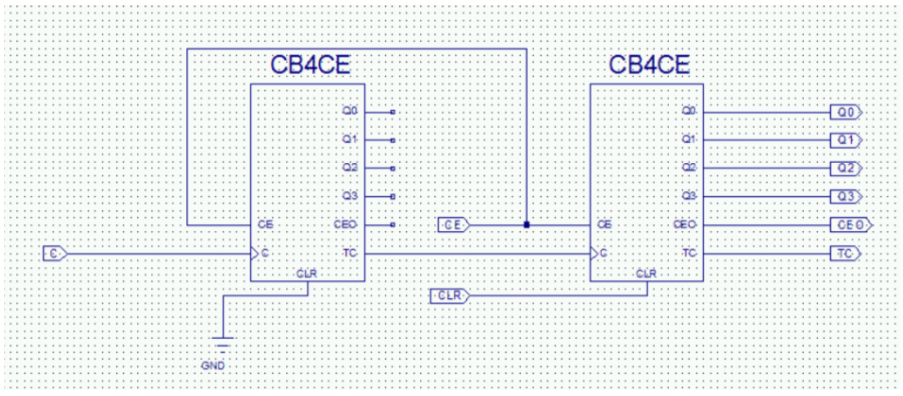
\includegraphics[ scale = 0.4]{auf_1_1.png}
  	\caption[Schaltskizze des 8fach-Zählers]{Schaltskizze des 8fach-Zählers}
  \label{fig:auf_1_1}
\end{figure}

Dabei werden die Aus- und Eingänge nach dem folgende Schema belegt.

\begin{figure}[H]
\centering
\begin{tabular}{|c|c|}
\hline Marker & Pin \\ \hline
\hline C & P6 \\ 
\hline CE & P2 \\ 
\hline CLR & P9 \\ 
\hline TC & P24 \\ 
\hline CEO & P22 \\ 
\hline Q0 & P12 \\ 
\hline Q1 & P13 \\ 
\hline Q2 & P14 \\ 
\hline Q3 & P18 \\ 
\hline 
\end{tabular} 
\end{figure}

\subsubsection*{Versuchsdurchführung}
%erklären, !was! wir machen, !warum! wir das machen und mit welchem ziel
%(wichtig) präzize erklären, wie bei dem versuch vorgegangen und was gemacht wurde

Es wird über die Mitte Pinreihe CLK ein Jumper gesetzt. Dann wird Pinreihen SV1 mit SW über ein Flachbandkabel verbunden so wie SV2 mit LED. Danach wird mit SW1 überprüft, ob die Schaltung funktioniert und mit SW8 der Zählzustand wieder zurückgesetzt und das Flachbandkabel zwischen SV2 und LED wieder entfernt. Und über SV12 das Board an das Oszilloskop angeschlossen. Dann werden mit dem Oszillsokop die Frequenzen von Q0 bis Q3 gemessen.

\subsubsection*{Messergebnisse}
%die messwerte in !übersichtlichen! tabellen angegeben
%zu viele kleine tabellen in große tabellen überführen!
%zu große tabellen mit dem [scale]-befehl scalieren oder (falls zu lang) in zwei kleinere tabellen aufteilen
%(wichtig) vor !jeder! tabelle sagen, was gemessen wurde und wie die fehler gewählt wurden und ausreichend !erklären!, !warum! wir unsere fehler grade so gewählt haben

Die Werte wurden direkt vom Oszillskop abelesen.

\begin{figure}[H]
\centering
\begin{tabular}{|c|c|}
\hline Ausgang & Frequenz/kHz \\ \hline
\hline Q0 & 3 \\ 
\hline Q1 & 1,2 \\ 
\hline Q2 & 0,6 \\ 
\hline Q3 & 0,6 \\ 
\hline 
\end{tabular} 
\end{figure}


\subsubsection*{Auswertung}
%zuerst !alle! errechneten werte entweder in ganzen sätzen aufzählen, oder in tabellen (übersichtlicher) dargestellen, sowie auf die verwendeten formeln verweisen (die referenzierung der formel kann in der überschrift stehen)
%kurz erwähnen (vor der tabelle), warum wir das ganze ausrechnen bzw. was wir dort ausrechnen
%danach histogramme und plots erstellen, wobei wenn möglich funktionen durch die plots gelegt werden (zur not können auch splines benutzt werden, was aber angegeben werden muss)
%bei fits immer die funktion und das reduzierte chiquadrat mit angegeben, wobei auf verständlichkeit beim entziffern der zehnerpotenzen geachtet werden muss z.b. f(x)=(wert+-fehler)\cdot10^{irgendeine zahl}\cdot x + (wert+-fehler)\cdot10^{irgendeine zahl}
%bei jedem fit erklären, nach welchem zusammenhang gefittet wurde und warum!
%bei plots darauf achten, dass die achsenbeschriftung (auch die tics) die richtige größe haben und die legende im plot nicht die messwerte verdeckt
%kurz die aufgabenstellung abhandeln
%2-----------------------------------------------2

Da in dem Aufbau ein CD4CE und kein CB4CE verwendet wrude sind die Messergebnisse nicht wie gewünscht auswertbar. Der CD4CE zählt lediglich bis von 0 bis 9 und nicht wie gewünscht von 0 bis 15. Das ist auch in der Aufnahme (Abbildung \ref{fig:frequ_1}) der Ausgangsfrequenzen zu sehen.

\begin{figure}[H] 
  \centering 	
    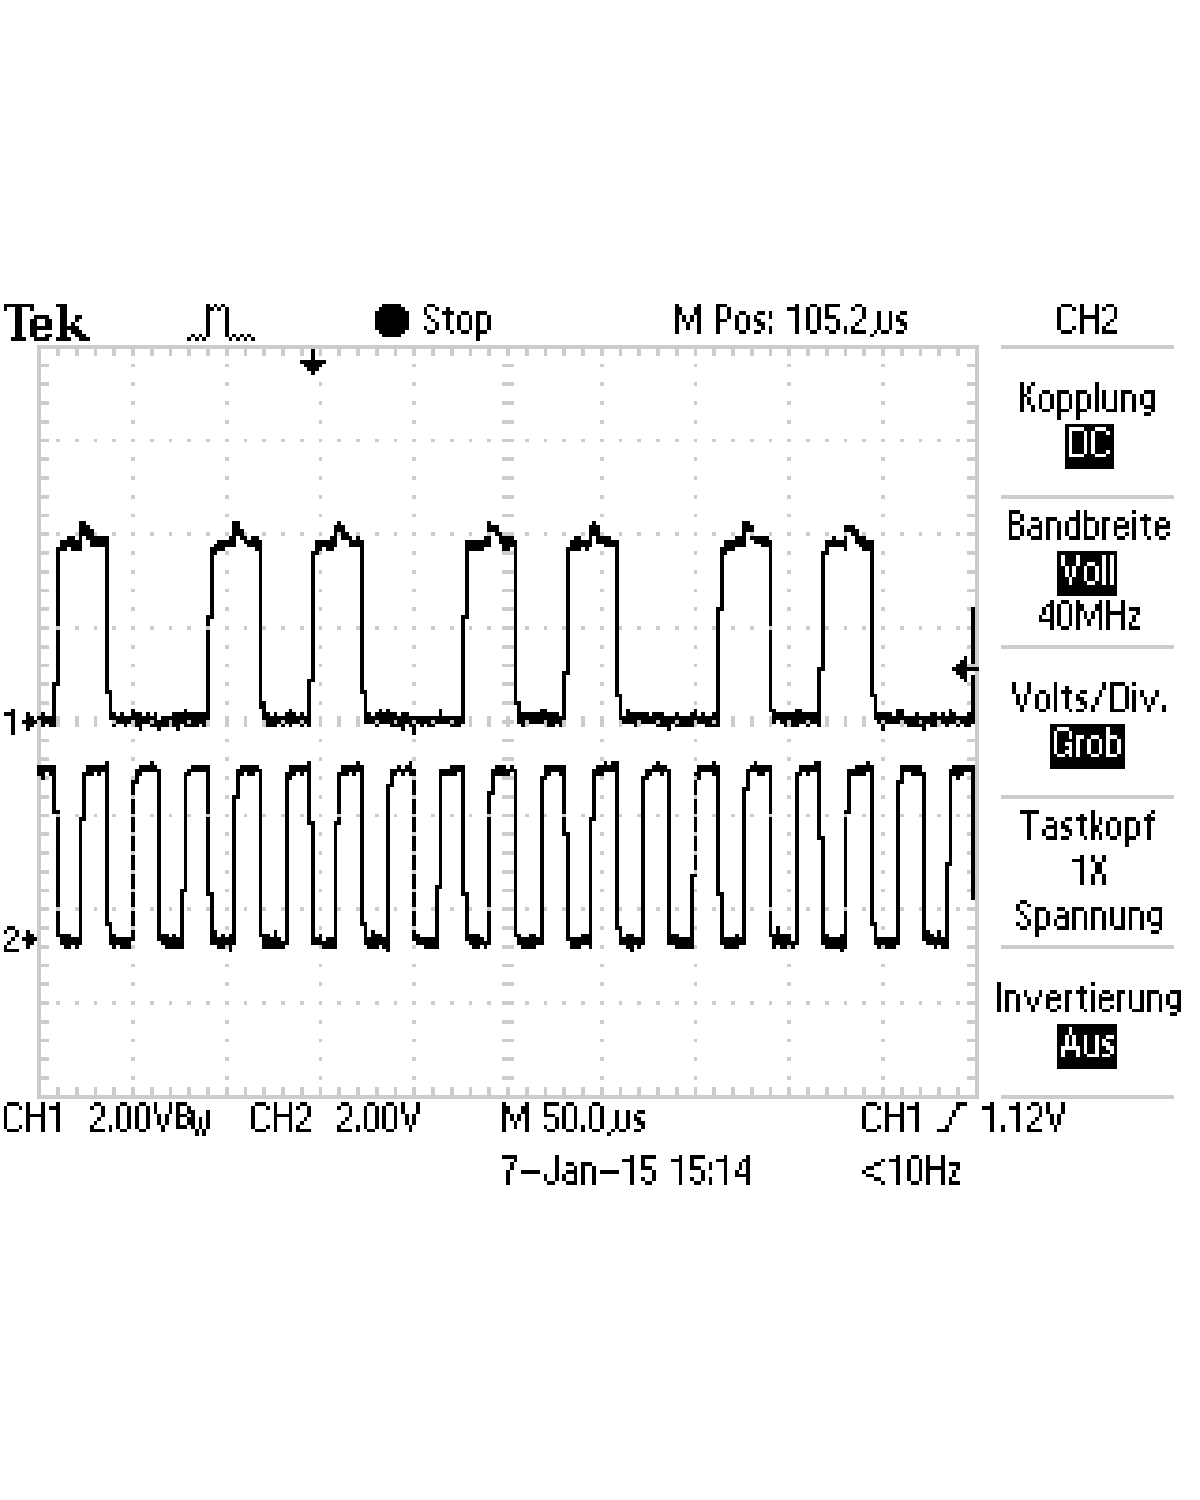
\includegraphics[trim = 0mm 50mm 0mm 50mm, clip, scale = 0.4]{TEK0011.pdf}
  	\caption[Aufnahme des Ausgangsfrequenz]{Aufnahme des Ausgangsfrequenz}
  \label{fig:frequ_1}
\end{figure}

Es wurde erwartet, dass auf immer nur Abfallende Flanke auf einander liegen.

\subsection{Änderungen der Schaltung (1): 16fach-Zähler}
%kurz das ziel dieses versuchsteiles ansprechen, damit keine zwei überschriften direkt übereinander stehen!
%bei schwierigeren versuchen kann auch der theoretische hintergrund erläutert werden. (mit formeln, herleitungen und erklärungen)

In diesem Versuchsteil soll die Eingangsfrequenz von 50kHz auf 1Hz herabgeseng werden. Dafür wird die selbe Schaltung wie in dem vorherigen Versuchsteil verwendet, jedoch werden vier anstatt zwei CB4CE hintereinander geschaltet.

\subsubsection*{Verwendete Geräte}
%(immer) eine skizze oder ein foto einfügen, die geräte/materialien !nummerieren! und z.b. eine legende dazu schreiben, besser wäre es das ganze in einem Fließtext gut zu beschreiben.
%falls am anfang des versuches nicht klar ist, was alles verwendet wird, wenn möglich erst am ende ein großes foto von den verwendeten materialien machen!\\

Es werden das CPLD-Board, Verbindungskabel und ein Oszilloskop verwendet.

\subsubsection*{Versuchsaufbau}
%skizze zum versuchsaufbau (oder foto) einfügen,   es muss erklärt werden wie das ganze funktioniert und welche speziellen einstellungen verwendet wurden (z.b. welche knöpfe an den geräten für die messung verdreht wurden)

Es wird die Schaltung in Abbildung \ref{fig:auf_1_1} mit ISE aufgebaut und implementiert.

\begin{figure}[H] 
  \centering 	
    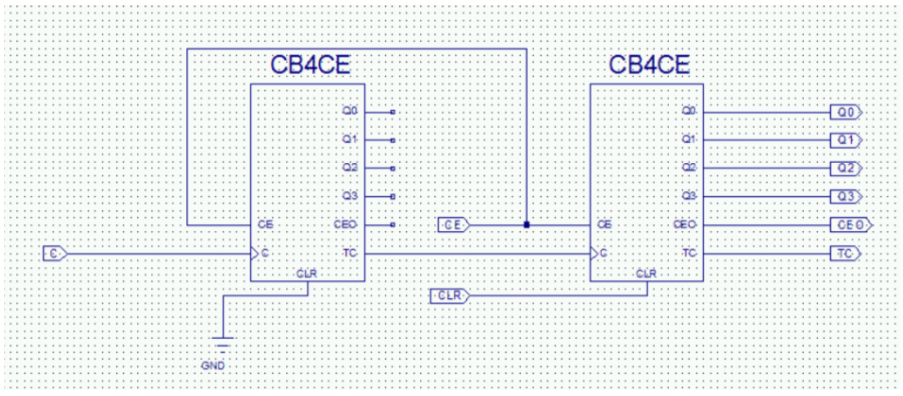
\includegraphics[ scale = 0.4]{auf_1_1.png}
  	\caption[Schaltskizze des 16fach-Zählers]{Schaltskizze des 16fach-Zählers}
  \label{fig:auf_1_1}
\end{figure}

Dabei werden die Aus- und Eingänge nach dem folgende Schema belegt.

\begin{figure}[H]
\centering
\begin{tabular}{|c|c|}
\hline Marker & Pin \\ \hline
\hline C & P6 \\ 
\hline CE & P2 \\ 
\hline CLR & P9 \\ 
\hline TC & P24 \\ 
\hline CEO & P22 \\ 
\hline Q0 & P12 \\ 
\hline Q1 & P13 \\ 
\hline Q2 & P14 \\ 
\hline Q3 & P18 \\ 
\hline 
\end{tabular} 
\end{figure}


\subsubsection*{Versuchsdurchführung}
%erklären, !was! wir machen, !warum! wir das machen und mit welchem ziel
%(wichtig) präzize erklären, wie bei dem versuch vorgegangen und was gemacht wurde

Es wird Pinreihen SV1 mit SW über ein Flachbandkabel verbunden. Danach wird  über SV12 das Board an das Oszilloskop angeschlossen und mit dem Oszillsokop die Periodendauer von Q0 bis Q3 gemessen. Es wird die Periodendauer gemessen, da das Oszilloklop keine Frequenzen unter 10Hz messen kann.

\subsubsection*{Messergebnisse}
%die messwerte in !übersichtlichen! tabellen angegeben
%zu viele kleine tabellen in große tabellen überführen!
%zu große tabellen mit dem [scale]-befehl scalieren oder (falls zu lang) in zwei kleinere tabellen aufteilen
%(wichtig) vor !jeder! tabelle sagen, was gemessen wurde und wie die fehler gewählt wurden und ausreichend !erklären!, !warum! wir unsere fehler grade so gewählt haben

Die Messwerte wurde direkt vom Oszillsokop abgelesen.

\begin{figure}[H]
\centering
\begin{tabular}{|c|c|}
\hline Ausgang & Periodendauer/ms \\ \hline
\hline Q0 & 56 \\ 
\hline Q1 & 112 \\ 
\hline Q2 & 222 \\ 
\hline Q3 & 444 \\ 
\hline 
\end{tabular}
\label{tab:periode} 
\end{figure}

\subsubsection*{Auswertung}
%zuerst !alle! errechneten werte entweder in ganzen sätzen aufzählen, oder in tabellen (übersichtlicher) dargestellen, sowie auf die verwendeten formeln verweisen (die referenzierung der formel kann in der überschrift stehen)
%kurz erwähnen (vor der tabelle), warum wir das ganze ausrechnen bzw. was wir dort ausrechnen
%danach histogramme und plots erstellen, wobei wenn möglich funktionen durch die plots gelegt werden (zur not können auch splines benutzt werden, was aber angegeben werden muss)
%bei fits immer die funktion und das reduzierte chiquadrat mit angegeben, wobei auf verständlichkeit beim entziffern der zehnerpotenzen geachtet werden muss z.b. f(x)=(wert+-fehler)\cdot10^{irgendeine zahl}\cdot x + (wert+-fehler)\cdot10^{irgendeine zahl}
%bei jedem fit erklären, nach welchem zusammenhang gefittet wurde und warum!
%bei plots darauf achten, dass die achsenbeschriftung (auch die tics) die richtige größe haben und die legende im plot nicht die messwerte verdeckt
%kurz die aufgabenstellung abhandeln
%2-----------------------------------------------2

Bei der Messung der Periodendauer ergaben sich auf dem Ozillsokop für die Ausgänge Q0 und Q1 der Verlauf in Abbildung \ref{fig:periode_1}.

\begin{figure}[H] 
  \centering 	
    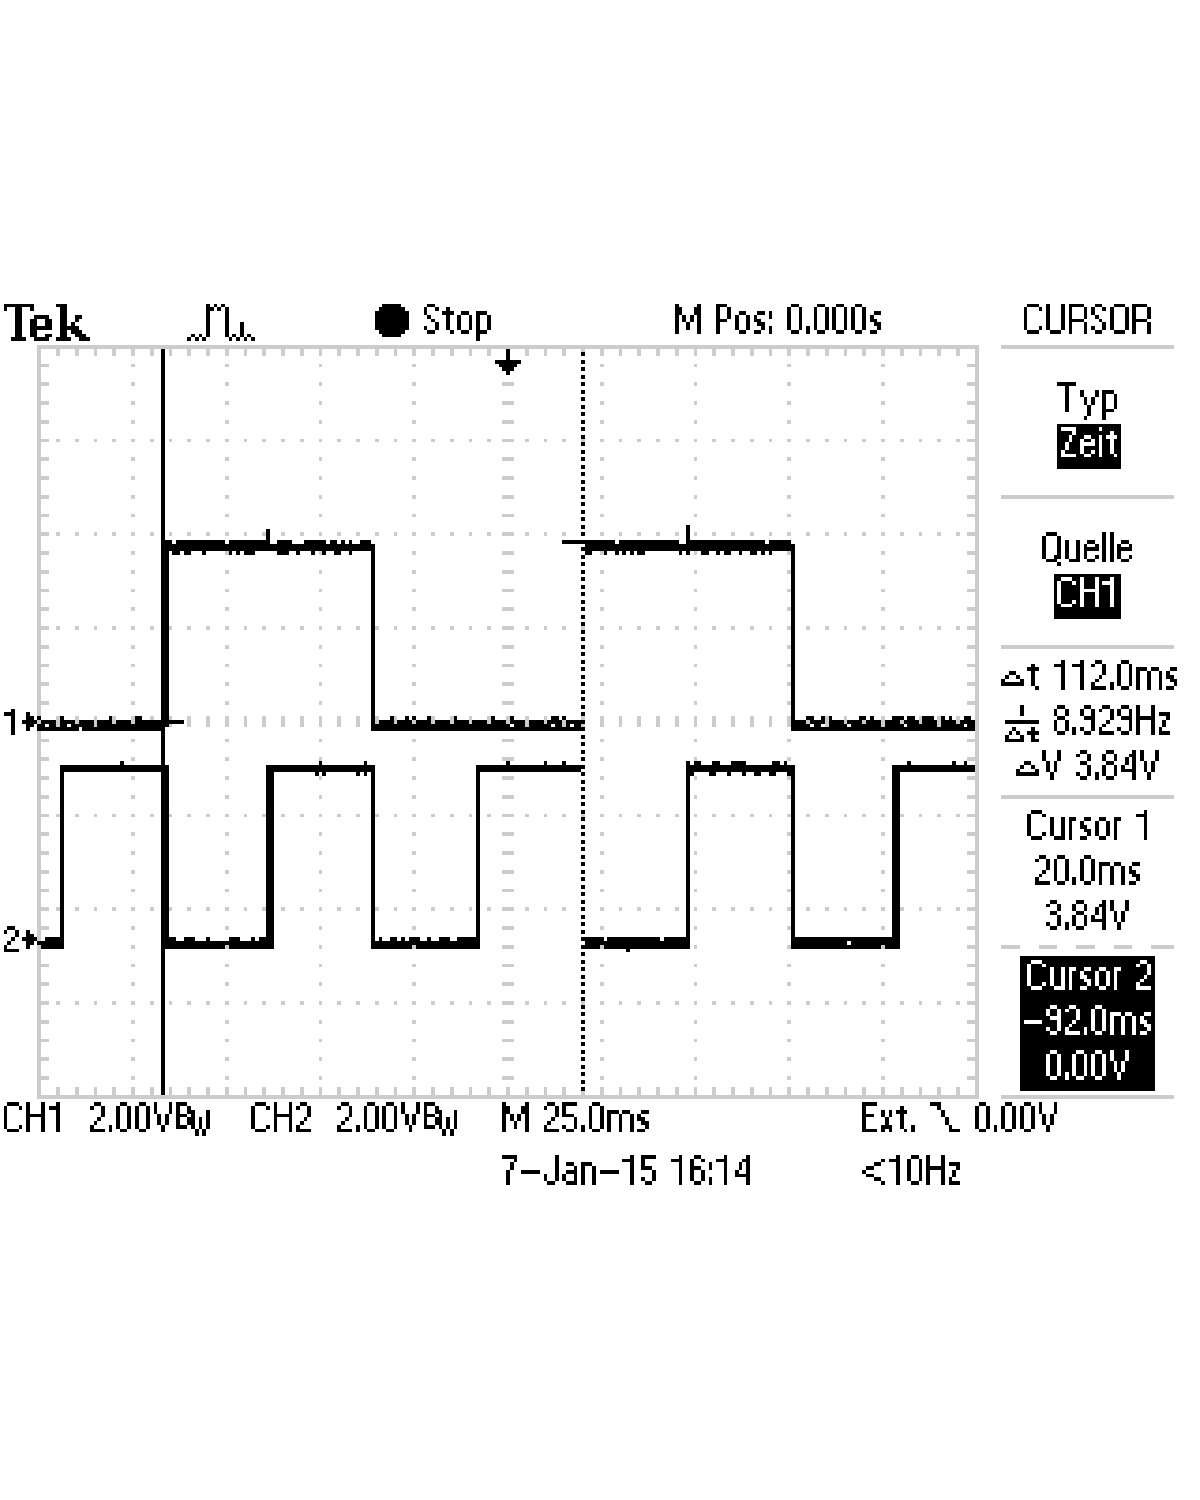
\includegraphics[trim = 0mm 50mm 0mm 50mm, clip, scale = 0.4]{TEK0012.pdf}
  	\caption[Aufnahme der Periodendauern für Q0 und Q1]{Aufnahme der Periodendauern für Q0 und Q1} 
  \label{fig:periode_1}
\end{figure}

Die Aufnahme auf dem Oszillsokop für Q2 und Q3 ist in Abbildung \ref{fig:periode_2} zu sehen.

\begin{figure}[H] 
  \centering 	
    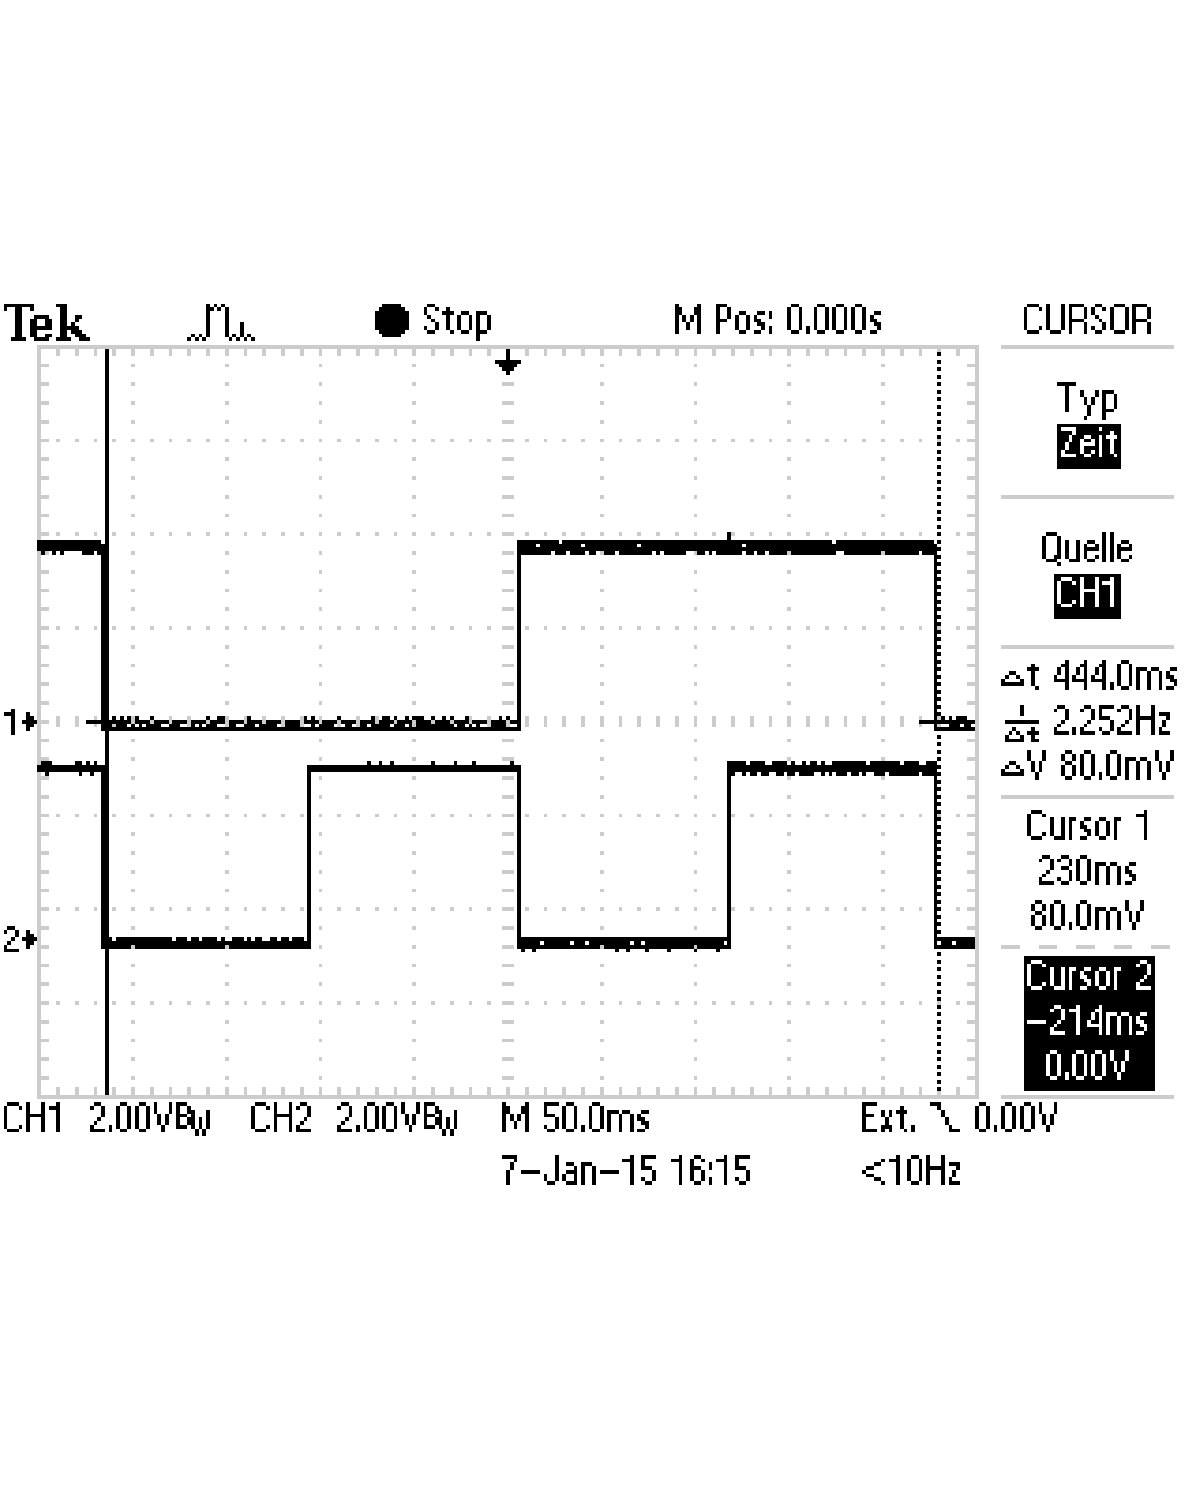
\includegraphics[trim = 0mm 50mm 0mm 50mm, clip, scale = 0.4]{TEK0013.pdf}
  	\caption[Aufnahme der Periodendauern für Q2 und Q3]{Aufnahme der Periodendauern für Q2 und Q3}
  \label{fig:periode_2}
\end{figure}

Es wurde erwartet, dass die sich die Frequenz zum nächsten Ausgang halbiert, dies ist anhand von Tabelle \ref{tab:periode} gut zu sehen. Die Frequenz und die Periodendauer hängen reziprok zusammen, daher entspricht eine verdoppelung der Periodendauer einer halbierung der Frequenz.

\subsection{Änderungen der Schaltung (2): 3-nach-8-Dekoder}
%kurz das ziel dieses versuchsteiles ansprechen, damit keine zwei überschriften direkt übereinander stehen!
%bei schwierigeren versuchen kann auch der theoretische hintergrund erläutert werden. (mit formeln, herleitungen und erklärungen)

Es sollen die hintersten drei Ausgänge so umprogrammiert werden dass nacheinander die acht Leuchtdioden angehen.

\subsubsection*{Verwendete Geräte}
%(immer) eine skizze oder ein foto einfügen, die geräte/materialien !nummerieren! und z.b. eine legende dazu schreiben, besser wäre es das ganze in einem Fließtext gut zu beschreiben.
%falls am anfang des versuches nicht klar ist, was alles verwendet wird, wenn möglich erst am ende ein großes foto von den verwendeten materialien machen!\\

Es werden das CPLD-Board, Verbindungskabel und ein PC verwendet.

\subsubsection*{Versuchsaufbau}
%skizze zum versuchsaufbau (oder foto) einfügen,   es muss erklärt werden wie das ganze funktioniert und welche speziellen einstellungen verwendet wurden (z.b. welche knöpfe an den geräten für die messung verdreht wurden)

\label{subsec:aufbau}

Es wird die Schaltung in Abbildung \ref{fig:auf_1_1} mit ISE aufgebaut und implementiert.

\begin{figure}[H] 
  \centering 	
    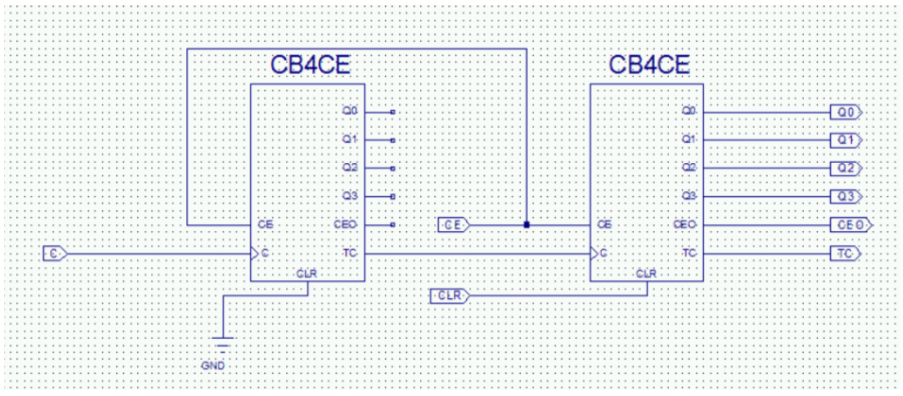
\includegraphics[ scale = 0.4]{auf_1_1.png}
  	\caption[Schaltskizze des 16fach-Zählers]{Schaltskizze des 16fach-Zählers}
  \label{fig:auf_1_1}
\end{figure}

Dabei werden die Aus- und Eingänge nach dem folgende Schema belegt.

\begin{figure}[H]
\centering
\begin{tabular}{|c|c|c|}
\hline CPLD & SV3 & LED \\ \hline
\hline 1 & 1 & 1 \\ 
\hline 44 & 2 & 2 \\ 
\hline 42 & 3 & 3 \\ 
\hline 43 & 4 & 4 \\ 
\hline 40 & 5 & 5 \\ 
\hline 39 & 6 & 6 \\ 
\hline 38 & 7 & 7 \\ 
\hline 37 & 8 & 8 \\ 
\hline 
\end{tabular} 
\end{figure}


\subsubsection*{Versuchsdurchführung}
%erklären, !was! wir machen, !warum! wir das machen und mit welchem ziel
%(wichtig) präzize erklären, wie bei dem versuch vorgegangen und was gemacht wurde

Es wird die Schaltung wie in im Abschnitt \ref{subsec:aufbau} aufgebaut und implementiert, dann wird das Verhalten der LEDs beobachtet.

\subsubsection*{Auswertung}
%zuerst !alle! errechneten werte entweder in ganzen sätzen aufzählen, oder in tabellen (übersichtlicher) dargestellen, sowie auf die verwendeten formeln verweisen (die referenzierung der formel kann in der überschrift stehen)
%kurz erwähnen (vor der tabelle), warum wir das ganze ausrechnen bzw. was wir dort ausrechnen
%danach histogramme und plots erstellen, wobei wenn möglich funktionen durch die plots gelegt werden (zur not können auch splines benutzt werden, was aber angegeben werden muss)
%bei fits immer die funktion und das reduzierte chiquadrat mit angegeben, wobei auf verständlichkeit beim entziffern der zehnerpotenzen geachtet werden muss z.b. f(x)=(wert+-fehler)\cdot10^{irgendeine zahl}\cdot x + (wert+-fehler)\cdot10^{irgendeine zahl}
%bei jedem fit erklären, nach welchem zusammenhang gefittet wurde und warum!
%bei plots darauf achten, dass die achsenbeschriftung (auch die tics) die richtige größe haben und die legende im plot nicht die messwerte verdeckt
%kurz die aufgabenstellung abhandeln
%2-----------------------------------------------2

Es war zu beobachten, dass die Schaltung wie erwartet die LEDs der Reihen nach hochzählte.

\subsubsection*{Diskussion}
%(immer) die gemessenen werte und die bestimmten werte über die messfehler mit literaturwerten oder untereinander vergleichen
%in welchem fehlerintervall des messwertes liegt der literaturwert oder der vergleichswert?
%wie ist der relative anteil des fehlers am messwert und damit die qualität unserer messung?
%in einem satz erklären, wie gut unser fehler und damit unsere messung ist
%kurz erläutern, wie systematische fehler unsere messung beeinflusst haben könnten
%(wichtig) zum schluss ansprechen, in wie weit die ergebnisse mit der theoretischen vorhersage übereinstimmen
%--------------------------------------------------------------------------------------------
%falls tabellen mit den messwerten zu lang werden, kann die section mit den messwerten auch hinter der diskussion angefügt bzw. eine section mit dem anhang eingefügt werden.
%1-----------------------------------------------1

Im ersten Versuchsteil konnten leider nicht die gewünschen Ergebnisse erzielt werden da ein falschen Bauteil verwendet wurde. In den anderen beiden Versuchteilen sind gut ergebnisse erzielt worden und es konnte bestätigt werden, was erwartet wurde.

\section{Programmierung der CPLD mit der Hardware Description Language Verilog}
%kurz das ziel dieses versuchsteiles ansprechen, damit keine zwei überschriften direkt übereinander stehen!
%bei schwierigeren versuchen kann auch der theoretische hintergrund erläutert werden. (mit formeln, herleitungen und erklärungen)
Da das Erstellen des Schaltplanes bei komplizierteren Schaltungen sehr mühsam wird, ist es einfacher die Schaltung mit einer HDL (Verilog) zu programmieren. Ziel dieses Versuchsteiles ist es, einen Vorzähler (12 bis 16 Bit) und einen 8-Bit-Zähler zu programmieren, welcher dann auf den 8 LEDs und den beiden Sibensegmentanzeigen angezeigt werden soll. Dafür müssen jeweils 4 Bits des Zählers in einen 8-Bit-Zustand der Siebensegmentanzeige übergeführt werden.
\subsection*{Verwendete Geräte}
%(immer) eine skizze oder ein foto einfügen, die geräte/materialien !nummerieren! und z.b. eine legende dazu schreiben, besser wäre es das ganze in einem Fließtext gut zu beschreiben.
%falls am anfang des versuches nicht klar ist, was alles verwendet wird, wenn möglich erst am ende ein großes foto von den verwendeten materialien machen!\\
Verwendet werden ein Computer, das CPLD, ein Programmieradapter, eine 9V Spannungsquelle sowie nach Versuchsteil mehrere Flachbandkabel.
\subsection{Ein neues Projekt}
%kurz das ziel dieses versuchsteiles ansprechen, damit keine zwei überschriften direkt übereinander stehen!
%bei schwierigeren versuchen kann auch der theoretische hintergrund erläutert werden. (mit formeln, herleitungen und erklärungen)
Diesmal soll ein neues Projekt nicht über einen Schaltplan, sondern über eine Verilog Datei definiert werden.
Die genaue Vorgehensweise kann in der Versuchsbeschreibung nachgelesen werden.\footnote{http://www.atlas.uni-wuppertal.de/$\sim$kind/ep9\_14.pdf Seite 19 und 20}
\subsection{Ein einfaches Verilog Programm für die 8 LEDs}
%kurz das ziel dieses versuchsteiles ansprechen, damit keine zwei überschriften direkt übereinander stehen!
%bei schwierigeren versuchen kann auch der theoretische hintergrund erläutert werden. (mit formeln, herleitungen und erklärungen)
Am CPLD wird die Pinreihe SV1 mit der Pinreihe SW verbunden, sowie die Pinreihe SV2 mit der Pinreihe LED. Dazu werden zwei Flachbandkabel verwendet. Es wird nun ein Vorgegebenes Programm kompiliert und dessen Funktion untersucht.
\subsubsection*{Versuchsaufbau}
%skizze zum versuchsaufbau (oder foto) einfügen,   es muss erklärt werden wie das ganze funktioniert und welche speziellen einstellungen verwendet wurden (z.b. welche knöpfe an den geräten für die messung verdreht wurden)
Es wird der Quellcode \ref{scr:1} aus der Versuchsanleitung übernommen, kompiliert und dessen Funktion beobachtet.
\subsubsection*{Versuchsdurchführung}
%erklären, !was! wir machen, !warum! wir das machen und mit welchem ziel
%(wichtig) präzize erklären, wie bei dem versuch vorgegangen und was gemacht wurde
Nachdem ein neues Projekt erstellt wurde (vgl. Versuchsanleitung S. 19 f.), wird der in der Versuchsanleitung angegebene Programmiercode eingefügt. Der Programmiercode ist bereits auskommentiert. Nachdem die Syntax überprüft wurde, kann das Programm kompiliert werden. Nach weiteren Arbeitsschritten (vgl. Versuchsanleitung S. 22) sollte auf den 8 LEDs das Binärmuster des hochlaufenden Zählers angezeigt werden.

\subsubsection*{Auswertung}
%zuerst !alle! errechneten werte entweder in ganzen sätzen aufzählen, oder in tabellen (übersichtlicher) dargestellen, sowie auf die verwendeten formeln verweisen (die referenzierung der formel kann in der überschrift stehen)
%kurz erwähnen (vor der tabelle), warum wir das ganze ausrechnen bzw. was wir dort ausrechnen
%danach histogramme und plots erstellen, wobei wenn möglich funktionen durch die plots gelegt werden (zur not können auch splines benutzt werden, was aber angegeben werden muss)
%bei fits immer die funktion und das reduzierte chiquadrat mit angegeben, wobei auf verständlichkeit beim entziffern der zehnerpotenzen geachtet werden muss z.b. f(x)=(wert+-fehler)\cdot10^{irgendeine zahl}\cdot x + (wert+-fehler)\cdot10^{irgendeine zahl}
%bei jedem fit erklären, nach welchem zusammenhang gefittet wurde und warum!
%bei plots darauf achten, dass die achsenbeschriftung (auch die tics) die richtige größe haben und die legende im plot nicht die messwerte verdeckt
%kurz die aufgabenstellung abhandeln
%2-----------------------------------------------2
Das Programm konnte erfolgreich kompiliert werden. 
Es wurde beobachtet, dass die LEDs im Binärsystem Hochzählen.
\subsection{Änderung 1:Ausgabe des Zählers an die Siebensegmentanzeigen}
%kurz das ziel dieses versuchsteiles ansprechen, damit keine zwei überschriften direkt übereinander stehen!
%bei schwierigeren versuchen kann auch der theoretische hintergrund erläutert werden. (mit formeln, herleitungen und erklärungen)
In diesem Versuchsteil soll der Zählerstand auf der Siebensegmentanzeige sichtbar gemacht werden.
\subsubsection*{Versuchsaufbau}
%skizze zum versuchsaufbau (oder foto) einfügen,   es muss erklärt werden wie das ganze funktioniert und welche speziellen einstellungen verwendet wurden (z.b. welche knöpfe an den geräten für die messung verdreht wurden)
Die Pinreihe SV3 wird mit einem weiteren Flachbandkabel mit der Pinreihe DIS1 verbunden.
Der Quellcode aus der Versuchsanleitung wurde während des Versuches konfiguriert (Code \ref{scr:2}).
\subsubsection*{Versuchsdurchführung}
%erklären, !was! wir machen, !warum! wir das machen und mit welchem ziel
%(wichtig) präzize erklären, wie bei dem versuch vorgegangen und was gemacht wurde
Im Quellcode werden die voher auskommentierten Register 'segments1' und 'segments2' aktiviert. Am Ende des always Blocks wird ein vorgegebener Befehl hinzugefügt. Danach wird der Quellcode kompiliert und die Funktion der Siebensegmentanzeige überprüft.
\textbf{Fragen}:
\begin{itemize}
\item Wie kann die Geschwindigkeit erhöht oder erniedrigt werden, mit der die Zählerzustände durchlaufen werden, ohne die Eingangsfrequenz (ca. 50 kHz) zu verändern?
\item Das Signal CLR dient zum Rücksetzen des Zählers. Welcher Taster erzeugt es?
\item Ein weiteres Signal wurde bisher gar nicht benutzt: CE (clock enable). Wie kann Sie es erreichen, daß der Zähler nur läuft, wenn CE auf 1 ist? Wie kann man den Zähler stoppen, wenn CE auf 1 ist? Welcher Taster erzeugt CE?
\end{itemize} 
\begin{enumerate}
\item Die Geschwindigkeit, mit der die Zählerzustände durchlaufen werden, ändert sich mit der Größe der Variablen 'prescaler' (momentan 14 Bit). 15 Bit halbiert die Geschwindigkeit, 13 Bit verdoppelt sie.
\item Der Taster SW8 in der Ecke oben rechts auf dem Board ist CLR und dient zum zurücksetzen des Zählers.
\item Für CE kann eine zusätzliches If Kommando in das Programm eingefügt werden, welche den Zähler beinhaltet. Diese Funktion wurde jedoch erst im letzten Versuchsteil in den Quellcode eingebaut. CE liegt auf dem Taster SW1, und der Zähler kann, wie wir im letzten Versuchsteil sehen werden, mit CLR gestoppt werden, wenn CE auf 1 ist.
\end{enumerate}
\subsubsection*{Auswertung}
%zuerst !alle! errechneten werte entweder in ganzen sätzen aufzählen, oder in tabellen (übersichtlicher) dargestellen, sowie auf die verwendeten formeln verweisen (die referenzierung der formel kann in der überschrift stehen)
%kurz erwähnen (vor der tabelle), warum wir das ganze ausrechnen bzw. was wir dort ausrechnen
%danach histogramme und plots erstellen, wobei wenn möglich funktionen durch die plots gelegt werden (zur not können auch splines benutzt werden, was aber angegeben werden muss)
%bei fits immer die funktion und das reduzierte chiquadrat mit angegeben, wobei auf verständlichkeit beim entziffern der zehnerpotenzen geachtet werden muss z.b. f(x)=(wert+-fehler)\cdot10^{irgendeine zahl}\cdot x + (wert+-fehler)\cdot10^{irgendeine zahl}
%bei jedem fit erklären, nach welchem zusammenhang gefittet wurde und warum!
%bei plots darauf achten, dass die achsenbeschriftung (auch die tics) die richtige größe haben und die legende im plot nicht die messwerte verdeckt
%kurz die aufgabenstellung abhandeln
%2-----------------------------------------------2
nachdem der Quellcode konfiguriert und kompiliert wurde, konnte beobachtet werden, dass an der 7-Segmentanzeige zuerst die 0, dann die 1 und danach jede einzelne der 8 LEDs aufleuchteten. Der If-Befehl für CE wurde erst im letzten Versuchsteil eingebaut.
\subsection{Änderung 2:Strichmuster für alle 16 Zustände}
%kurz das ziel dieses versuchsteiles ansprechen, damit keine zwei überschriften direkt übereinander stehen!
%bei schwierigeren versuchen kann auch der theoretische hintergrund erläutert werden. (mit formeln, herleitungen und erklärungen)
In diesem Versuchsteil soll die Siebensegmentanzeige die Zahlen 0-f des Hexadezimalsystems darstellen.
\subsubsection*{Versuchsaufbau}
%skizze zum versuchsaufbau (oder foto) einfügen,   es muss erklärt werden wie das ganze funktioniert und welche speziellen einstellungen verwendet wurden (z.b. welche knöpfe an den geräten für die messung verdreht wurden)
Der Quellcode aus der Versuchsanleitung wurde während des Versuches konfiguriert (Code \ref{scr:3}).
\subsubsection*{Versuchsdurchführung}
%erklären, !was! wir machen, !warum! wir das machen und mit welchem ziel
%(wichtig) präzize erklären, wie bei dem versuch vorgegangen und was gemacht wurde
Die Zahlen 1-f im Hexadezimalsystem sollen mit den 8 Bits des Siebensegmentdecoders dargestellt werden. Der case-Befehl weist jedem der 16 Zustände von 'decodeinput' (4 Bit) ein 8 Bit Muster, welches die LEDs am Siebensegmentdecoder aufleuchten lässt, zu. Nun sollen diese Muster im Quellcode verändert werden, sodass von 0 bis f hochgezählt wird.

\subsubsection*{Auswertung}
%zuerst !alle! errechneten werte entweder in ganzen sätzen aufzählen, oder in tabellen (übersichtlicher) dargestellen, sowie auf die verwendeten formeln verweisen (die referenzierung der formel kann in der überschrift stehen)
%kurz erwähnen (vor der tabelle), warum wir das ganze ausrechnen bzw. was wir dort ausrechnen
%danach histogramme und plots erstellen, wobei wenn möglich funktionen durch die plots gelegt werden (zur not können auch splines benutzt werden, was aber angegeben werden muss)
%bei fits immer die funktion und das reduzierte chiquadrat mit angegeben, wobei auf verständlichkeit beim entziffern der zehnerpotenzen geachtet werden muss z.b. f(x)=(wert+-fehler)\cdot10^{irgendeine zahl}\cdot x + (wert+-fehler)\cdot10^{irgendeine zahl}
%bei jedem fit erklären, nach welchem zusammenhang gefittet wurde und warum!
%bei plots darauf achten, dass die achsenbeschriftung (auch die tics) die richtige größe haben und die legende im plot nicht die messwerte verdeckt
%kurz die aufgabenstellung abhandeln
%2-----------------------------------------------2
Die Strichmuster konnten erfolgreich konfiguriert werden, der Zähler zählt von 0 bis f.
\subsection{Änderung 3: Aus dem Binärzähler wird ein Dezimalzähler}
%kurz das ziel dieses versuchsteiles ansprechen, damit keine zwei überschriften direkt übereinander stehen!
%bei schwierigeren versuchen kann auch der theoretische hintergrund erläutert werden. (mit formeln, herleitungen und erklärungen)
In diesem Versuchsteil soll die Siebensegmentanzeige nach der Zahl '9' wieder bei '0' anfangen zu zählen.
\subsubsection*{Versuchsaufbau}
%skizze zum versuchsaufbau (oder foto) einfügen,   es muss erklärt werden wie das ganze funktioniert und welche speziellen einstellungen verwendet wurden (z.b. welche knöpfe an den geräten für die messung verdreht wurden)
Der Quellcode aus der Versuchsanleitung wurde während des Versuches konfiguriert (Code \ref{scr:4}).
\subsubsection*{Versuchsdurchführung}
%erklären, !was! wir machen, !warum! wir das machen und mit welchem ziel
%(wichtig) präzize erklären, wie bei dem versuch vorgegangen und was gemacht wurde
In die always-Schleife wird wie in der Versuchsbeschreibung beschrieben ein If-Befehl, welcher 'counter[3:0]' bei 'counter[3:0] == 10' innerhalb dieser auf 0 setzt, eingefügt, sodass nach der '9' wieder die '0' am Siebensegmentdecoder angezeigt wird.  
\subsubsection*{Auswertung}
%zuerst !alle! errechneten werte entweder in ganzen sätzen aufzählen, oder in tabellen (übersichtlicher) dargestellen, sowie auf die verwendeten formeln verweisen (die referenzierung der formel kann in der überschrift stehen)
%kurz erwähnen (vor der tabelle), warum wir das ganze ausrechnen bzw. was wir dort ausrechnen
%danach histogramme und plots erstellen, wobei wenn möglich funktionen durch die plots gelegt werden (zur not können auch splines benutzt werden, was aber angegeben werden muss)
%bei fits immer die funktion und das reduzierte chiquadrat mit angegeben, wobei auf verständlichkeit beim entziffern der zehnerpotenzen geachtet werden muss z.b. f(x)=(wert+-fehler)\cdot10^{irgendeine zahl}\cdot x + (wert+-fehler)\cdot10^{irgendeine zahl}
%bei jedem fit erklären, nach welchem zusammenhang gefittet wurde und warum!
%bei plots darauf achten, dass die achsenbeschriftung (auch die tics) die richtige größe haben und die legende im plot nicht die messwerte verdeckt
%kurz die aufgabenstellung abhandeln
%2-----------------------------------------------2
Der If-Befehl wurde an der passenden Stelle im Quellcode eingefügt und sorgt dafür, dass nur noch von 0 bis 9 hochgezählt wird. Die Funktion des Quellcodes wurde nach dem programmieren des CPLD an Siebensegmentdecoder beobachtet.
\subsection{Änderung 4: Ein zweistelliger Zähler}
%kurz das ziel dieses versuchsteiles ansprechen, damit keine zwei überschriften direkt übereinander stehen!
%bei schwierigeren versuchen kann auch der theoretische hintergrund erläutert werden. (mit formeln, herleitungen und erklärungen)
Es soll nun ein zweistelliger Zähler implementiert werden, welcher von '00' bis '99' hochzählt. Daneben wird auch die Funktion des CE Tasters, welche im zweiten Versuchsteil angesprochen wurde, implementiert.
\subsubsection*{Versuchsaufbau}
%skizze zum versuchsaufbau (oder foto) einfügen,   es muss erklärt werden wie das ganze funktioniert und welche speziellen einstellungen verwendet wurden (z.b. welche knöpfe an den geräten für die messung verdreht wurden)
Die Pinreihe SV4 wird mit einem Flachbandkabel mit der Pinreihe DIS2 verbunden.
Der Quellcode aus der Versuchsanleitung wurde während des Versuches konfiguriert (Code \ref{scr:5} und Code \ref{scr:6}).
\subsubsection*{Versuchsdurchführung}
%erklären, !was! wir machen, !warum! wir das machen und mit welchem ziel
%(wichtig) präzize erklären, wie bei dem versuch vorgegangen und was gemacht wurde
Zuerst wird ein zweites 4 Bit Register counter2 hinzugefügt.
Danach wird die always-Schleife verändert. Falls CLR gedrückt wird, soll ebenfalls counter2 (neben dem Prescaler und counter) auf null gesetzt werden.\\
\textbf{Frage}:
\begin{itemize}
\item Wenn Sie den CLR-Taster drücken, springt das Siebensegmentdisplay nicht sofort auf Null. Warum? Wie können Sie das ändern?
\end{itemize}
\begin{enumerate}
\item
Damit das Siebensegmentdisplay auf null springt muss dahinter 'segments1' und 'segments2' mit der segment7-Funktion sowie den Registern 'conter[3:0]' für 'segments1' und 'counter2[3:0]' für 'segments2'  das entsprechende 8 Bitmuster zugewiesen werden. Dies wird erst im letzten Teil des Quellcodes eingefügt, sodass CLR davor zum Anhalten des Zählers benutzt werden kann.
\end{enumerate}
Nun soll der Zähler nur laufen, falls CE gedrückt gehalten wird. Dafür wird anstatt 'else begin ... end' der Befehle 'else if(CE) begin ... end' implementiert. In dem Befehl 'if(counter[3:0] == 10) begin ... end' muss jetzt zusätzlich 'counter2' um 1 erhöht werden. Damit counter2 nicht von 0 bis f, sondern von 0 bis 9 hochzählt, wird ein weiterer If-Befehl ergänzt, welcher die gleiche Struktur hat, wie der für counter, sodass an der Siebensegmentanzeige nach '99' wieder '00' angezeigt wird. Zum Schluss soll neben 'segments1' auch 'segments2' das richtige 8 Bitmuster zugewiesen werden. Also wird neben 'segments1' auch 'segments2' mit der Funktion segment7 das passende 8 Bitmuster zugewiesen. (In diesem Fall das von counter2)
Falls es zu Fehlermeldungen wegen den Ressourcen des CPLD kam, wurden die Größen der Register angepasst.
\subsubsection*{Auswertung}
%zuerst !alle! errechneten werte entweder in ganzen sätzen aufzählen, oder in tabellen (übersichtlicher) dargestellen, sowie auf die verwendeten formeln verweisen (die referenzierung der formel kann in der überschrift stehen)
%kurz erwähnen (vor der tabelle), warum wir das ganze ausrechnen bzw. was wir dort ausrechnen
%danach histogramme und plots erstellen, wobei wenn möglich funktionen durch die plots gelegt werden (zur not können auch splines benutzt werden, was aber angegeben werden muss)
%bei fits immer die funktion und das reduzierte chiquadrat mit angegeben, wobei auf verständlichkeit beim entziffern der zehnerpotenzen geachtet werden muss z.b. f(x)=(wert+-fehler)\cdot10^{irgendeine zahl}\cdot x + (wert+-fehler)\cdot10^{irgendeine zahl}
%bei jedem fit erklären, nach welchem zusammenhang gefittet wurde und warum!
%bei plots darauf achten, dass die achsenbeschriftung (auch die tics) die richtige größe haben und die legende im plot nicht die messwerte verdeckt
%kurz die aufgabenstellung abhandeln
%2-----------------------------------------------2
Der Quellcode konnte nach kurzer Zeit angepasst werden, sodass auf der Siebensegmentanzeige von '00' bis '99' hochgezählt wird. Da zu diesem Zeitpunkt die Anzeige mit CLR lediglich angehalten wurde, sollte der Quellcode danach so verändert werden, dass die Anzeige auf '00' springt, sobald CLR gedrückt wird. Dafür wurde am Ende des if(CLR)-Befehls 'segments1' und 'segments2' das entsprechende 8 Bitmuster zugewiesen.

\subsubsection*{Diskussion}
%(immer) die gemessenen werte und die bestimmten werte über die messfehler mit literaturwerten oder untereinander vergleichen
%in welchem fehlerintervall des messwertes liegt der literaturwert oder der vergleichswert?
%wie ist der relative anteil des fehlers am messwert und damit die qualität unserer messung?
%in einem satz erklären, wie gut unser fehler und damit unsere messung ist
%kurz erläutern, wie systematische fehler unsere messung beeinflusst haben könnten
%(wichtig) zum schluss ansprechen, in wie weit die ergebnisse mit der theoretischen vorhersage übereinstimmen
%--------------------------------------------------------------------------------------------
%falls tabellen mit den messwerten zu lang werden, kann die section mit den messwerten auch hinter der diskussion angefügt bzw. eine section mit dem anhang eingefügt werden.
%1-----------------------------------------------1
Verilog konnte in diesem Versuch ohne große Schwierigkeiten verwendet werden.
Die einzelnen Konfigurationsschritte konnten alle umgesetzt werden und nach dem programmieren des CPLD an den leuchtenden LEDs der LED-Anzeige und der bzw. den beiden Anzeigen der Siebensegmentdecoder überprüft werden. Es stellte sich je nach Aufgabenteil das erwartete Ergebnis ein.

\section{Fazit}
%im fazit nochmal alles zusammenfassen und den verlauf der messung abschätzen
%gravierende sytematische probleme bei den messungen nochmal betonen und die wertigkeit unserer ergebnisse einordnen
Bis auf einen kleinen Fehler am Anfang des Versuches, der uns sehr viel Zeit gekostet hat, ist der Versuch gut verlaufen. Am Ende war leider keine Zeit mehr für die Bearbeitung der Zusatzaufgabe über.

\section{Anhang}

Im Anhang befinden sich die jeweils verwendeten Verilogdateien und die ufc Datei, die die Pinbelegung angibt.

\begin{figure}[H]
\lstinputlisting[, basicstyle=\tiny]{ufc.ufc}
\caption*{Datei zur Festlegung der Pinbelegung}
\label{scr:1}
\end{figure}

\begin{figure}[H]
\lstinputlisting[language=Verilog, basicstyle=\tiny]{Verilog_1_iso.v}
\caption*{Quellcode für die 1. Aufgabe}
\label{scr:1}
\end{figure}


\newpage

\begin{figure}[H]
\lstinputlisting[language=Verilog, basicstyle=\tiny]{Verilog_2.v}
\caption*{Quellcode für die 2. Aufgabe}
\label{scr:2}
\end{figure}


\newpage

\begin{figure}[H]
\lstinputlisting[language=Verilog, basicstyle=\tiny]{Verilog_3.v}
\caption*{Quellcode für die 3. Aufgabe}
\label{scr:3}
\end{figure}


\newpage

\begin{figure}[H]
\lstinputlisting[language=Verilog, basicstyle=\tiny]{Verilog_4.v}
\caption*{Quellcode für die 4. Aufgabe}
\label{scr:4}
\end{figure}


\newpage

\begin{figure}[H]
\lstinputlisting[language=Verilog, basicstyle=\tiny]{Verilog_6.v}
\caption*{Quellcode für die 5. Aufgabe}
\label{scr:5}
\end{figure}

\newpage

\begin{figure}[H]
\lstinputlisting[language=Verilog, basicstyle=\tiny]{Verilog_7.v}
\caption*{Quellcode für die 5. Aufgabe}
\label{scr:6}
\end{figure}




\end{document}